\eat{
  Execution Feedback
  Instruction Feedback
  Machine feedback
  Human feedback
}

\section{LLMs and RL}

In this section, we discuss some connections
between RL and
``\keywordDef{foundation models}''
(see e.g., \citep{foundationModels}).
These are large pretrained
generative models of text and/or images
such as  \keywordDef{large language models} (\keywordDef{LLMs})
and their multimodal extension,
sometimes called
\keywordDef{vision language models} (\keywordDef{VLMs}).
Note that this is a very fast growing field, so we
only briefly mention a few highlights.
For more details, see e.g.
\url{https://github.com/WindyLab/LLM-RL-Papers}.

  
\subsection{RL for LLMs}


We can think of LLMs as agents, where the state $s_t$
is the entire sequence of previous words,
$s_t = (w_1,\ldots,w_{t-1})$,
the action is the next word $w_{t}$\footnote{
%
When using VLMs, the ``words'' are a tokenized
representation of the visual input and/or output.
Even when using language, the elementary components
$w_t$ are sub-words (which allows for generalization),
not words.
So a more precise term would be ``tokens'' instead of ``words''.
},
the stochastic policy $\pi(a_t|s_t)$ is the LLM,
and the transition model is the determistic function
$p(s_{t+1}|s_t,a_t) = \delta(s_t=\text{concat}(s_t,a_t))$.
We see that the size of the state
grows linearly over time, which is a standard way to capture
non-local dependencies in a Markov model.  


  
We discuss how to train these models below.
Once trained, they are used in a semi-MDP fashion, in which
at round $t$ the agent
generates an answer $a_t = (a_{t,1},\ldots, a_{t,N_t})$,
which is a sequence of $N_t$ tokens,
in response to a prompt from the user,
$p_t = (p_{t,1},\ldots, p_{t,M_t})$,
and the previous context (dialog history),
$c_t = (p_{1,1:M_1}, a_{1,1:N_1}, p_{2,1:M_2}, \ldots,  a_{t-1,1:N_{t-1}})$.
We can now define the state as the sequence of tokens   $s_t=(c_t,p_t)$.
Similarly, the action sequence $a_t$ can be flattened into a single atomic
(string-valued) action, since there is no
 intermediate feedback from the environment after each token is produced.\footnote{
 %
 The fact that
 the action (token) sequence
 is generated by an autoregressive policy
 inside the agent's head is an implementation detail,
 and not part of the problem specification;
 for example, the agent could instead use discrete diffusion
 to generate $a_t = (a_{t,1},\ldots, a_{t,N_t})$.
 }
Note that, if there is a single round of prompting
  and answering (as is often assumed during training), then 
  this is a contextual bandit problem
  rather  than a full MDP.
  In particular, the context is the string $p_t$ and the action is
  the string $a_t$.
However, in multi-turn dialog situations, the agent's actions
will affect the environment (i.e., the user's mental state, and hence
subsequent prompt $p_{t+1}$), turning it into a full MDP.
 



\subsubsection{RLHF}
\label{sec:RLHF}

LLMs are usually trained with behavior cloning,
i.e., MLE on a fixed dataset,
such as  a large text (and tokenized image)
corpus scraped from the web.
This is called ``\keywordDef{pre-training}''.
We can then improve their performance using RL, as we describe below;
this is called ``\keywordDef{post-training}''.

A common way to perform post-training is to use
\keywordDef{reinforcement learning from human feedback}
or \keywordDef{RLHF}.
This technique, which was first introduced in the \keyword{InstructGPT} paper
\citep{instructGPT}, works as follows.
First a large number of (context, answer0, answer1) tuples are generated,
either by a human or an LLM.
Then human raters are asked  if they prefer answer 0 or answer 1.
Let $y=0$ denote the event that they prefer answer 0, and $y=1$ the event
that they prefer answer 1.
We can then fit a model of the form
\be
p(y=0|a_0,a_1,c) = \frac{\exp(\phi(c, a_0))}
{\exp(\phi(c, a_0)) + \exp(\phi(c, a_1))}
\ee
using binary cross entropy loss,
where $\phi(c,a)$ is some function that maps text to a
scalar (interpreted as logits).
Typically $\phi(c,a)$ is a shallow MLP on top of the last layer
of a pretrained LLM.
Finally, we define the reward function as
$R(s,a)=\phi(s,a)$,
where $s$ is the context (e.g., a prompt or previous dialog state),
and $a$ is the action (answer generated by LLM).
We then use this reward to fine-tune the LLM using
a policy gradient method such as PPO (\cref{sec:PPO}),
or a simpler method such as \keywordDef{RLOO}
\citep{Ahmadian2024},
which is based on REINFORCE (\cref{sec:REINFORCE}).

\eat{
Note that RLHF is training a reward model
that works well for a contextual bandit,
and not necessarily for an RL agent.
To see this, let the context or state $s$ be the text prompt,
the action $a$ be the text  generated as an answer,
and the reward $R(s,a)$ be the RLHF model.
The LLM policy is updated to maximize this one-step reward.
However, in practice,
after taking an action (generating a text answer), the dialog
will usually continue, so the next state
will depend on the previous state.
The standard reward learning model does
}

Note that this form of training assumes the agent
just interacts with a single action (answer) in response to a single
prompt, so is learning the reward for a bandit problem, rather than the full MDP.
Also, the learned reward function is a
known parametric model (since it is fit to the human feedback data),
whereas in RL, the reward is
an unknown non-differentiable  blackbox function.
When viewed in this light, it becomes clear that one can also use
non-RL algorithms  to improve performance of LLMs,
such as \keywordDef{DPO} \citep{Rafailov2023}
or the density estimation methods of \citep{Dumoulin2024}.
For more details  on RL for LLMs,
see e.g., \citep{Kaufmann2023}.


\subsubsection{Assistance game}
\label{sec:assistance}

In general, any objective-maximizing agent may suffer from reward hacking (\cref{sec:hacking}),
even if the reward has been learned using lots of RLHF data.
In  \citep{Russell2019}, Stuart Russell proposed a clever solution to this problem.
Specifically, the human and machine are both treated as agents in a
two-player cooperative game, called an \keywordDef{assistance game},
where the machine's goal is to maximize
the user's utility (reward) function, which is inferred based  on the human's behavior
using inverse RL.
%
That is, instead of trying to learn a point estimate
of the reward function using RLHF, and then optimizing that,
we treat the reward function as an unknown part of the environment.
If we adopt a Bayesian perspective on this, we can maintain a posterior
belief over the model parameters.
This will incentivize
the agent to perform information gathering actions.
For example,  if the machine is uncertain about whether something is a good idea or not,
it will proceed cautiously (e.g., by asking the user for their preference),
rather than blindly solving the wrong problem.
For more details on this framework, see \citep{Shah2020assistance}.

\eat{
  % https://github.com/hyp1231/awesome-llm-powered-agent
  Text agent
  LLM agent: text states, text actions 
  Reasoning agent: internal action
}


\subsubsection{Run-time inference as MPC}

Recently the LLM community has investigated ways to improve
the ``reasoning'' performance  of LLMs by using MCTS-like methods
(see \cref{sec:MCTS}).
The basic idea is to perform Monte Carlo rollouts of many possible
action sequences (by generating different ``chains of thought''
in response to the context so far),
and then applying a  value function to the leaves of this search tree
to decide on which trajectory to return as the final ``decision''.
The value function is usually learned using policy gradient methods,
such as REINFORCE (see e.g., \citep{Zelikman2024}).
% https://github.com/hijkzzz/Awesome-LLM-Strawberry
It is believed that OpenAI's
recently released 
\keywordDef{o1} (aka \keywordDef{Strawberry}) model\footnote{
%
See \url{https://openai.com/index/learning-to-reason-with-llms/}.
}%
uses similar techniques,
most likely pre-training on large numbers of human reasoning traces.

Note that the resulting policy is an instance of MPC (\cref{sec:MPC})
or decision time planning.
This means that, as in MPC, the agent must replan
after every new state observation (which incorporates
the response from the user),  making the method much
slower than ``reactive'' LLM policies, that does not use look-ahead
search (but still conditions on the entire past context).
However, once trained, it may be possible to distill this slower ``system 2'' policy
into a faster reactive ``system 1'' policy.


\subsection{LLMs for RL}



There are many ways that (pretrained) LLMs can be used for RL,
by leveraging their prior knowledge,
their ability to generate code,
their ``reasoning'' ability,
and their ability to perform \keywordDef{in-context learning}
(which can be viewed as a form of Bayesian inference
\citep{Panwar2024}, which is a ``gradient-free'' way of
optimally learning that is well suited to 
rapid learning from limited data).
The survey in \citep{Cao2024} groups the literature into four main categories:
LLMs for pre-processing the inputs,
LLMs for rewards,
LLMs for world models,
and
LLMs for decision making or policies.
In our brief presentation below,
we follow this categorization.
(See also \citep{Spiegel2024} for a similar grouping.)

\subsubsection{LLMs for pre-processing the input}

If the input observations $\vo_t$ sent
to the agent are in natural language
(or some other textual representation, such as JSON),
it is natural to use an LLM to process them,
in order to compute a more compact
representation,  $\vs_t=\vphi(\vo_t)$,
where $\vphi$ can the hidden state of the last layer of an LLM.
This encoder can either be frozen, or fine-tuned with the policy
network.
Note that we can also pass in the entire past observation history,
$\vo_{1:t}$,
as well as  static ``side information'',
such as instruction manuals or human hints;
these can  all be concatenated to form the LLM prompt.

For example, the \keywordDef{AlphaProof} system\footnote{
%
See \url{https://deepmind.google/discover/blog/ai-solves-imo-problems-at-silver-medal-level/}.
} %
uses an LLM (called the ``formalizer network'')
to translate an informal specification of a math problem
into the formal Lean representation,
which is then passed to an agent (called the ``solver network'')
which is trained,
using the AlphaZero method (see \cref{sec:alphaZero}),
to generate proofs
inside the Lean theorem proving environment.
In this environment,  the reward is 0 or 1 
(proof is correct or not),
the state space is a structured set of previously proved facts
and the current goal,
and the action space is a set of proof tactics.
%Thus the agent is not itself an LLM;
%the LLM is just used to preprocess the input.
The agent itself   is a separate  transformer policy network
(distincy from the formalizer network)
that is trained from scratch in an incremental way,
based on the AlphaZero method.


If the observations are images,
it it is traditional to use a CNN to proccess the input,
so $\vs_t \in \real^N$ would be an embedding vector.
However, we could alternatively use a VLM
to compute a structured representation,
where $\vs_t$ might be a set of tokens
describing  the scene at a high level.
We then proceed as in the text case.

Note that the information that is extracted will heavily depend on the prompt
that is used.
Thus we should think of an LLM/VLM as an \keywordDef{active sensor}
that we can control via prompts.
Choosing how to control this sensor
requires expanding the action space of the agent
to include computational actions \citep{Chen2024vlm}.
Note also that these kinds of ``sensors'' are very expensive to invoke,
so an agent with some limits on its time and compute (which is all practical agents)
will need to  reason about the value of information
and the cost of computation.
This is called \keywordDef{metareasoning} \citep{Russell1991}.
Devising good ways to train agents to perform both computational actions (e.g., invoking
an LLM or VLM) and environment actions (e.g., taking a step in the environment
or calling a tool) is an open research problem.


\subsubsection{LLMs for rewards}
\label{sec:LLMreward}

It is difficult to design a reward function to cause an agent
to exhibit some desired behavior, as we discussed in \cref{sec:reward}.
Fortunately LLMs can often help with this task. We discuss a few
approaches below.

In \citep{Klissarov2024}, they present the \keywordDef{Motif} system,
that uses
an LLM in lieu of a human to provide preference judgements to an RLHF system.
In more detail, a pre-trained policy is used to collect trajectories,
from which pairs of states, $(\vo, \vo')$, are selected at random.
The LLM is then asked which state is preferable, thus generating
$(\vo, \vo', y)$ tuples, which can be used to train a binary classifier
from which a reward model is extracted,
as in \cref{sec:RLHF}.
In \citep{Klissarov2024}, the observations $\vo$ 
are text captions generated by the NetHack game,
but the same method could be applied to images if we
used a VLM instead of an LLM for learning the reward.
The learned reward model is then used as a shaping function
(\cref{sec:rewardShaping}) when training an agent
in the NetHack environment,
which has very sparse reward.



In \citep{eureka}, they present
the \keywordDef{Eureka} system,
that learns the reward using bilevel optimization,
%(\cref{sec:rewardMeta}),
with RL on the inner
loop and LLM-powered evolutionary search on the outer loop.
In particular, in the inner loop, given a candidate reward function $R_i$,
we use PPO to train a policy,
and then return a scalar quality score $S_i=S(R_i)$.
In the outer loop, we ask
an LLM to generate a new set of reward functions, $R_i'$,
given a population of old reward functions and their scores,
$(R_i,S_i)$, which  have been trained
and evaluated in parallel on a fleet of GPUs.
The prompt also includes the source code
of the environment simulator.
Each generated reward function $R_i$ is represented as a Python function,
that has access to the ground truth state of the underlying
robot simulator.
The resulting system is able to learn a complex reward function
that is sufficient to train a policy (using PPO) that
can control a simulated robot hand to perform various dexterous
manipulation tasks, including spinning a pen with its finger tips.
In \citep{Li2024mc}, they present
a somewhat related approach and apply it to Minecraft.

In \citep{Venuto2024}, they propose \keywordDef{code as reward},
in which they prompt a VLM with an initial and goal image,
and ask it to describe the corresponding sequence of tasks
needed to reach the goal.
They then ask the LLM 
to synthesize code that checks for  completion of each subtask
(based on processing of object properties, such as relative
location, derived from the image).
These reward functions are
then ``verified''
by applying them to
an offline set of expert and random trajectories;
a good reward function should allocate high reward to
the expert trajectories and low reward to the random ones.
Finally, the reward functions are 
used as auxiliary rewards inside an RL agent.


There are of course many other ways an LLM could be used to help
learn reward functions, and this remains an active area of research.

\subsubsection{LLMs for world models}

There are  many papers that use transformers
or diffusion models to represent the world model
$p(s'|s,a)$,  and learn them from data collected
by the agent, as we discussed in \cref{sec:WM}.
Here we focus our attention on ways to use
pre-trained foundation models as world models (WM).

\eat{
In principle it is possible to treat a pre-trained FM
as an implicit model of the form $p(s'|s,a)$
by sampling responses to a suitable prompt,
which encodes $s$ and $a$. However, this rarely works
out of the box. A better approach
is to train the model on data that is relevant to the domain
of interest.
}

\citep{unisim} presents \keywordDef{UniSim},
which is an action-conditioned video diffusion model
trained on large amounts of robotics and visual navigation data.
Combined with a VLM reward model, this can be used
for decision-time planning as follows:
sample  candidate action
trajectories from a proposal,
generate the corresponding images,
feed them to the reward model,
score the rollouts,
and then pick the best action from this set.
(Note that this is just standard MPC in image space with a
diffusion WM and a random shooting planning algorithm.)

 \citep{Tang2024}
 presents \keywordDef{WorldCoder},
 which takes a very different approach.
It prompts a frozen LLM to generate code to represent
the WM $p(s'|s,a)$, which it then uses inside of a planning
algorithm. The agent then executes this in the environment,
and passes back failed predictions to the LLM, asking
it to improve the WM.
(This is related to the Eureka reward-learning system
mentioned in \cref{sec:LLMreward}.)

There are of course many other ways an LLM could be used to help
learn world models, and this remains an active area of research.

\subsubsection{LLMs for policies}

Finally we turn to LLMs as policies.

One approach 
is to pre-train a special purpose
foundation model  on state-action sequences (using behavior cloning),
then sample the next action
from it using $a_t \sim p(a_t|o_t,h_{t-1})$,
where $o_t$ is the latest observation
and $h_{t-1}=(o_{1:t-1},a_{1:t-1})$ is the history.
See e.g., \keywordDef{Gato} model \citep{gato}
\keywordDef{RT-2} \citep{Zitkovich2023},
and \keywordDef{RoboCat} \citep{Bousmalis2023}.

\begin{figure}
\centering
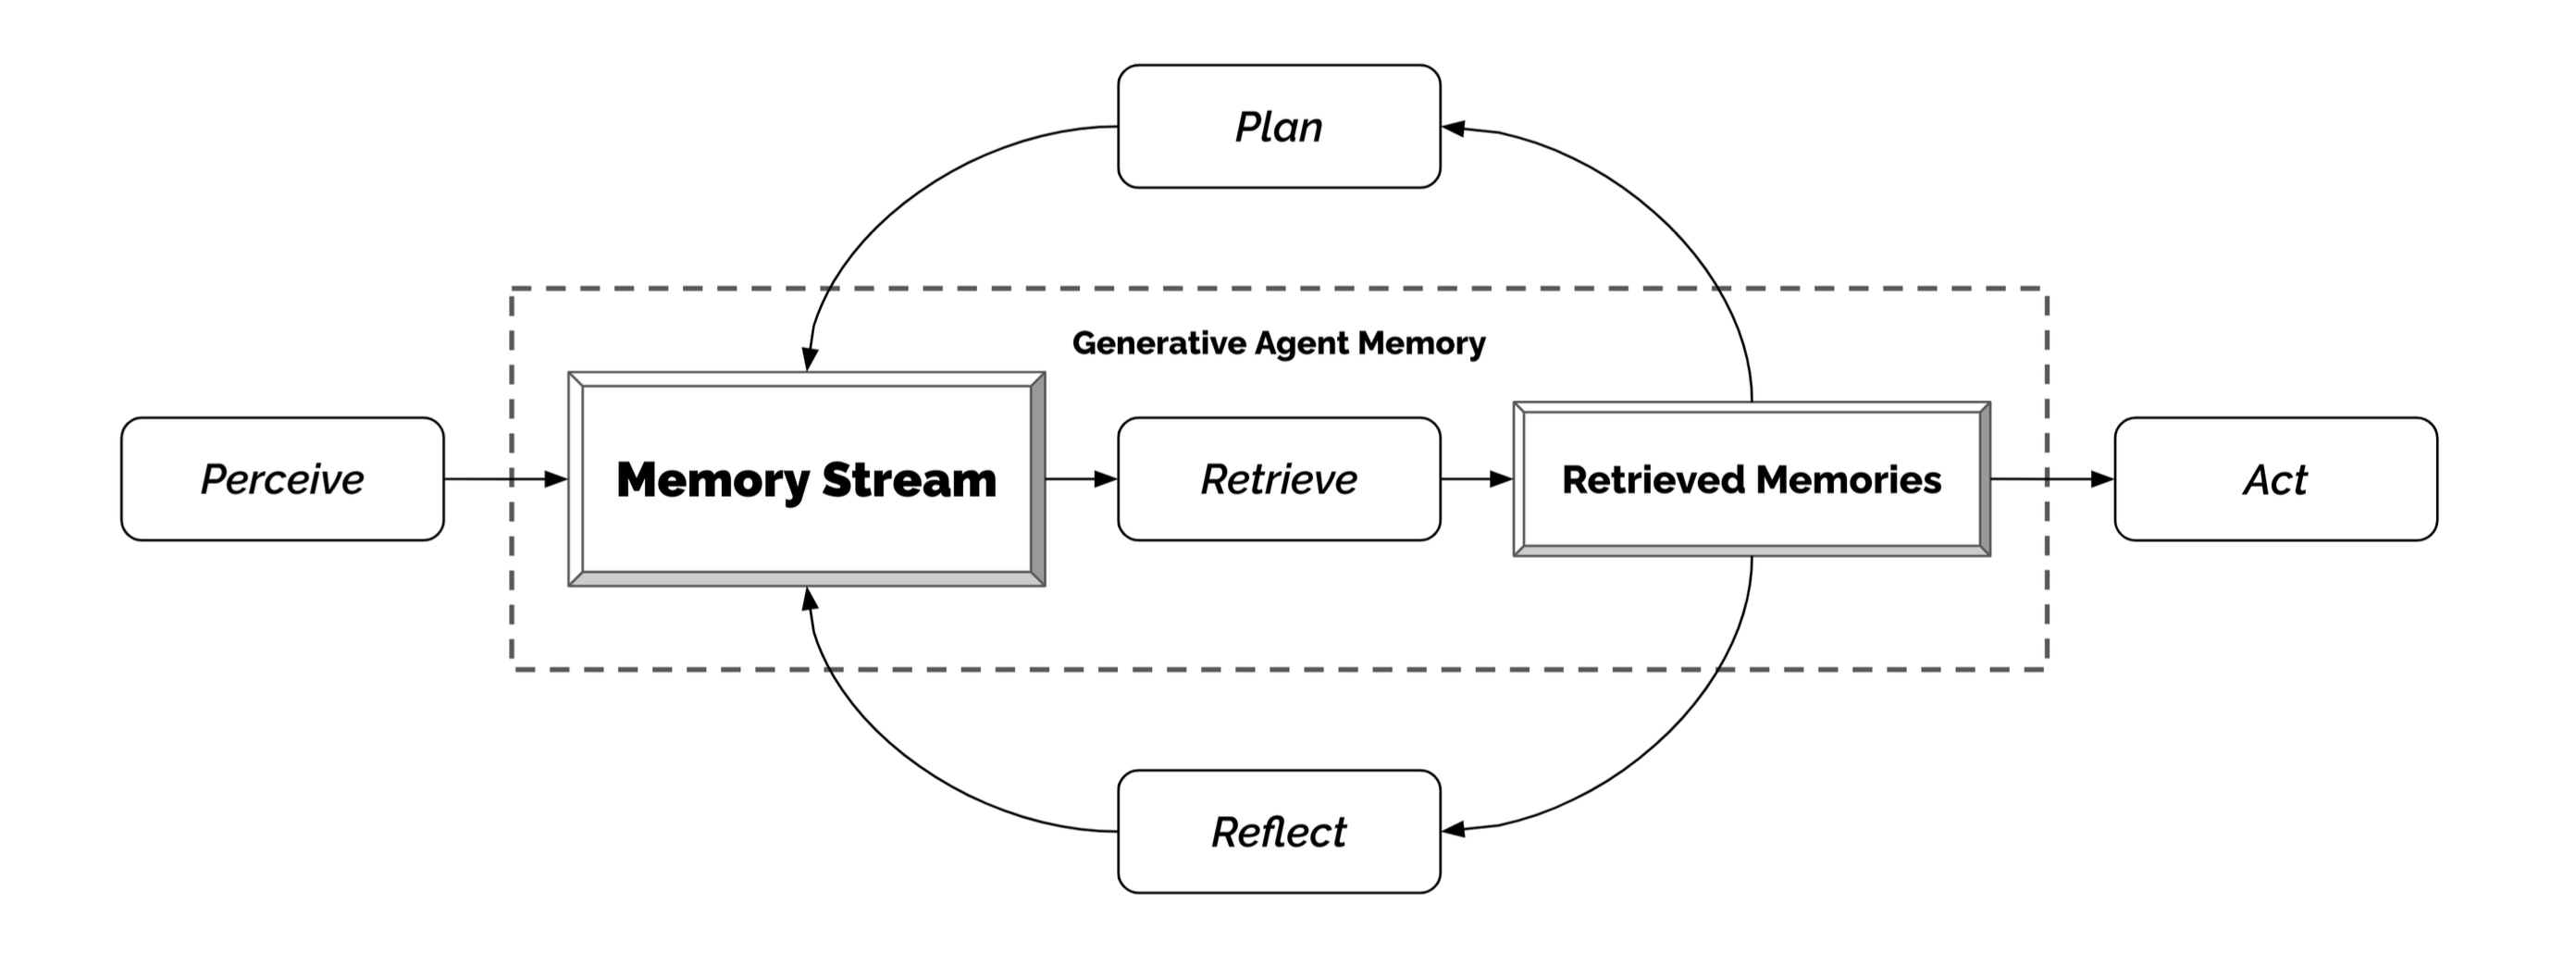
\includegraphics[height=2in]{figs/smallville}
\caption{
  Illustration of how to use a pretrained LLM (combined with RAG)
  as a policy.
  \figtaken{Figure 5 of \citep{Park2023}}.
  \figthanks{Joon Park}.
  }
\label{fig:smallville}
\end{figure}

More recently it has become popular to leverage
pre-trained LLMs that are trained on web data,
and then to repurpose them as ``agents'' using in-context learning.
We can then sample an action from the  policy $\pi(a_t|p_t,o_t,h_{t-1})$,
where $p_t$ is a  manually chosen prompt.
This approach is used by the \keywordDef{ReAct} paper
\citep{react} which 
works by prompting the LLM to ``think step-by-step''
(``reasoning'') and then to predict an action (``acting'').
This approach can be extended by prompting the LLM to first
retrieve relevant past examples from an external ``memory'',
rather than explicitly storing the entire history $h_t$ in the context
(this is called \keywordDef{retrieval augmented generation}
or \keywordDef{RAG}); see \cref{fig:smallville} for an illustration.
Note that no explicit learning (in the form of parametric updates)
is performed in these systems; instead they rely entirely
on in-context learning (and prompt engineering).


An alternative approach is to enumerate all possible
discrete actions, and use the LLM to  score them in terms
of their likelihoods given the goal,
and their suitability given a learned value function
applied to the current state,
i.e.  $\pi(a_t=k|g,p_t,o_t,h_t) \propto \text{LLM}(w_k|g_t,p_t,h_t) V_k(o_t)$,
where $g_t$ is the current goal,
$w_k$ is a text description of  action $k$,
and $V_k$ is the value function for action $k$.
This is the approach used in the
robotics \keywordDef{SayCan} approach \citep{Ichter2023},
where the primitive actions $a_k$ are  separately trained
goal-conditioned policies.

Calling the LLM at every step is very slow,
so an alternative is to use the LLM to generate
code that represents (parts of) the policy.
For example, the \keywordDef{Voyager} system in
\citep{voyager} builds up a reusable skill library
(represented as Python functions),
by alternating between environment exploration
and prompting the (frozen) LLM to generate new tasks and skills,
given the feedback collected so far.

There are of course many other ways an LLM could be used to help
learn policies, and this remains an active area of research.



